\chapter{Exact comparisons and perturbative reductions}
\label{narr:comparisons}

An ED eigenvalue, a quadratic matrix band, and a spin-response peak can all be
called a gap, yet they answer different questions. Perturbation theory adds
another distinction: the energy separation controlling an eliminated resolvent
is not automatically the excitation measured by a local probe. We make these
objects explicit before asking whether mean field agrees with an exact result.

% EDITORIAL QUESTION: Which gaps can differ even with identical energy units?
\section{Excitation energies and selection rules}
For the single block of Eq.~\eqref{eq:narr:one_mode}, occupation costs
$\varepsilon>0$, while the Hermitian matrix $\ii A$ has eigenvalues
$\pm\varepsilon$ separated by $2\varepsilon$. An ED spin gap is
$E_1-E_0$ in the physical spin space, with degeneracies and sector restrictions
specified. A probe onset is the smallest positive energy difference whose
matrix element for that probe is nonzero. A parity or symmetry rule can make
it larger than the lowest many-body excitation.

\begin{figure}[htbp]
\centering
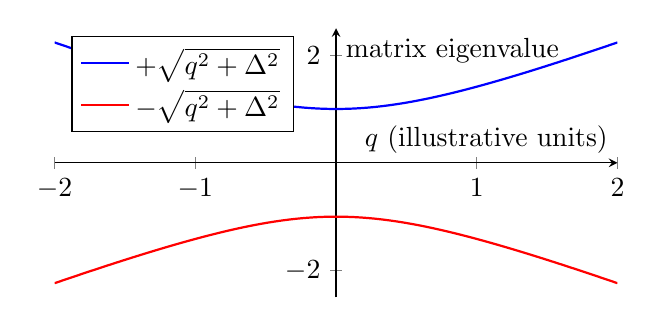
\begin{tikzpicture}
\begin{axis}[width=.72\textwidth,height=5cm,xlabel={$q$ (illustrative units)},
 ylabel={matrix eigenvalue},domain=-2:2,samples=80,axis lines=middle,
 ymin=-2.5,ymax=2.5,legend pos=north west]
\addplot[blue,thick]{sqrt(x*x+1)};
\addlegendentry{$+\sqrt{q^2+\Delta^2}$}
\addplot[red,thick]{-sqrt(x*x+1)};
\addlegendentry{$-\sqrt{q^2+\Delta^2}$}
\end{axis}
\end{tikzpicture}
\caption{An algebraic illustration with $\Delta=1$, not a fit or benchmark.
The smallest positive energy is $|\Delta|$, while the signed band separation
at $q=0$ is $2|\Delta|$. A physical probe threshold still needs a state space
and a matrix-element selection rule.}
\end{figure}

A cubic small-field mass mechanism does not fix its numerical coefficient.
The primary Kitaev derivation explicitly distinguishes a qualitative
scalar-denominator approximation from the full intermediate-state problem,
and retains a nonzero second-order time-reversal-even contribution. Its
third-order effective operators also include terms beyond a single bilinear
structure~\cite{Kitaev2006}. These facts rule out treating one assumed denominator
as an independently derived exact bulk prefactor.

% EDITORIAL QUESTION: Which projector is being eliminated in an exact reduction?
\section{Four projectors with different jobs}
% CLAIM: W001-FND-01 (note: doc/audits/w001_foundation_review.md).
On the physical zero-field Hilbert space let $P_{\rm ff}$ project onto the joint
zero-plaquette-flux sector, including all global Wilson sectors unless an extra
restriction is declared. Its complement $Q_{\rm flux}=\Id-P_{\rm ff}$ is the
block to be eliminated in a flux-sector reduction. A ground-eigenspace projector
$P_0$ is generally smaller. An external energy window
\begin{equation}
 P_\Lambda=P_{\rm ff}\,\mathbf1_{[E_0,E_0+\Lambda]}(H_0)
\end{equation}
restricts the external states; its full complement can also contain low-energy
flux-free matter states. Finally, $\Pi_{\rm occ}$ in
Chapter~\ref{narr:gaussian} acts in one-particle space. It cannot replace any
of these many-body projectors.

A single plaquette condition is not the joint flux-free condition when there
are multiple plaquettes. Likewise, sampling one pair-defect pattern does not
minimize over the entire eliminated block. If a sampled minimum is above the
true block edge, its reciprocal energy distance can \emph{underestimate} a
resolvent norm. Such sampling cannot certify an upper resolvent bound.

% EDITORIAL QUESTION: What is exact in the Feshbach map, and where do series assumptions enter?
\section{The conditional finite-dimensional reduction}
For a finite self-adjoint $H=H_0+\lambda V$, choose an orthogonal $P$ with
$[P,H_0]=0$ and $Q=\Id-P$. All inverses below are on $\Ran Q$. If
$E-QHQ$ is invertible, eliminating the $Q$ component of an eigenvector gives
\begin{equation}
 F(E,\lambda)=PHP+PHQ(E-QHQ)^{-1}QHP.
 \label{eq:narr:feshbach}
\end{equation}
This is an exact energy-dependent reduced operator. Write
$R_0=(E-QH_0Q)^{-1}$. A sufficient convergence condition for a fixed-energy
expansion is $|\lambda|\,\|QVQ R_0\|<1$, giving
\begin{equation}
 F=PH_0P+\lambda PVP+
 \sum_{r=0}^{\infty}\lambda^{r+2}PVQ R_0(QVQ R_0)^r QVP.
 \label{eq:narr:neumann}
\end{equation}
This statement has an explicit finite proof in Appendix~\ref{app:finite_foundations}.
It is not an evaluation of its coefficients on the honeycomb lattice.
An extensive perturbation norm may invalidate this sufficient criterion as
volume grows. A linked-cluster or locality argument would be additional work,
not a consequence of writing the finite series.

% EDITORIAL QUESTION: Does a vanishing first-order operator force second order to vanish?
\section{What symmetry does and does not remove}
% CLAIM: W001-FND-02 (note: doc/audits/w001_foundation_review.md).
If $P$ is the ground-eigenspace projector at energy $E_0$ with a positive gap
to $Q$, then $R_0$ at $E_0$ is negative on $\Ran Q$. Consequently
\begin{equation}
 \langle\psi|PVQ R_0 QVP|\psi\rangle
 =-\|(QH_0Q-E_0)^{-1/2}QV\psi\|^2\leq0,
 \qquad \psi\in\Ran P.
 \label{eq:narr:second_order}
\end{equation}
It vanishes for all external states exactly when $QVP=0$. The different
condition $PVP=0$ does not imply this. For example,
$H_0=\diag(0,\Delta)$, $P=\diag(1,0)$, $V=g\sigma_x$ gives
$PVP=0$ but second order $-g^2P/\Delta$.
A second-order energy shift may coexist with a third-order time-reversal-breaking
mass. Whether it is scalar or changes an effective dispersion is a further
model-specific question. The disapproved historical prefactor explanation
cannot be restored by conflating these orders or these observables.
